\begin{longtable}{p{0.5\textwidth} p{0.5\textwidth}}
  \tablesubsection{Beat Frequency}
   & \\
\end{longtable}
\begin{figure}[h!]
  \centering
  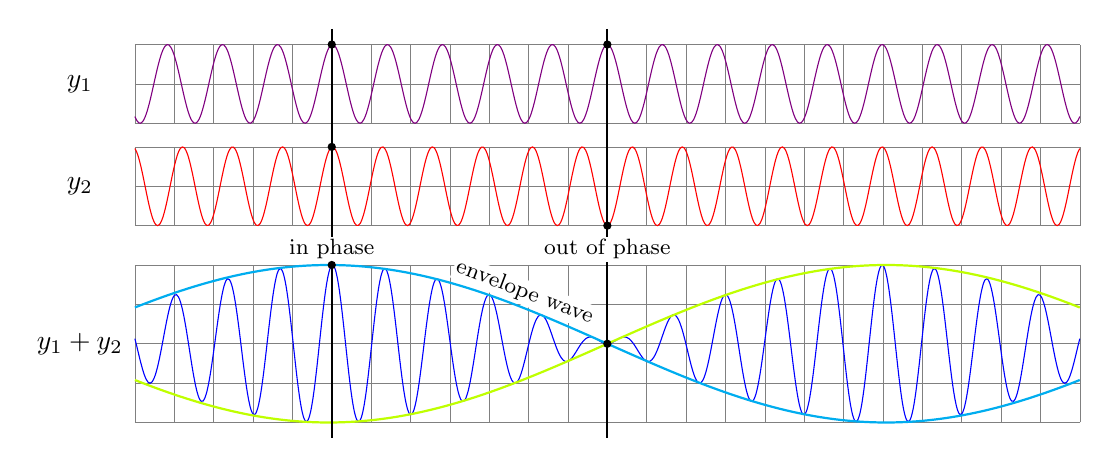
\begin{tikzpicture}
    
    % Grid
    \draw[step=0.5, very thin, gray] (-6,-0.5) grid ++(12, 1);
    \draw[step=0.5, very thin, gray, yshift=-1.3cm] (-6,-0.5) grid ++(12, 1);
    \draw[step=0.5, very thin, gray, yshift=-3.8cm] (-6,-0.5) grid ++(12, 2);
    
    % Graphs
    \draw[domain=-6:6,smooth,samples=500,variable=\x,violet] plot ({\x},{cos(deg(\x*9))/2});
    \draw[domain=-6:6,smooth,samples=500,variable=\x,red] plot ({\x},{-cos(deg(\x*9*1.1))/2-1.3});
    \draw[domain=-6:6,smooth,samples=500,variable=\x,blue] plot ({\x},{cos(deg(\x*9))/2-cos(deg(\x*9*1.1))/2-3.3});
    \draw[domain=-6:6,smooth,samples=500,variable=\x,lime, thick] plot ({\x},{2*sin(deg(\x*2*pi/9.9/1.43))/2-3.3});
    \draw[domain=-6:6,smooth,samples=500,variable=\x,cyan, thick] plot ({\x},{-2*sin(deg(\x*2*pi/9.9/1.43))/2-3.3});
    
    % Vertical lines
    \draw[-, thick] (-3.5, 0.7) -- (-3.5, -4.5);
    \draw[-, thick] (0, 0.7) -- (0, -4.5);
    
    % Nodes
    \draw (-6.7,0) node {$y_1$};
    \draw (-6.7,-1.3) node {$y_2$};
    \draw (-6.7,-3.3) node {$y_1+y_2$};
    \draw (-3.5,-2.1) node[fill=white,font=\footnotesize,inner sep=1pt] {in phase};
    \draw (0,-2.1) node[fill=white,font=\footnotesize,inner sep=1pt] {out of phase};
    \draw (-1.05,-2.65) node[fill=white,font=\footnotesize,inner sep=1pt,rotate=-21] {envelope wave};
    
    % Points
    \fill [black] (-3.5, 0.5) circle (1.5pt);
    \fill [black] (-3.5, -0.8) circle (1.5pt);
    \fill [black] (-3.5, -2.3) circle (1.5pt);
    
    \fill [black] (0, 0.5) circle (1.5pt);
    \fill [black] (0, -1.8) circle (1.5pt);
    \fill [black] (0, -3.3) circle (1.5pt);
    
  \end{tikzpicture}
  \caption{A diagram of the beat frequency between the waves $y_1$ and $y_2$ as traveling in the same direction where the beat frequency $f_b=\abs{f_2-f_1}$. The nodes of the combined wave occur where $y_1$ and $y_2$ are out of phase|that is, they have opposite amplitudes---and the antinodes of the combined wave occur where $y_1$ and $y_2$ are in phase---that is, they have equal amplitudes}
  \label{fig:beat-frequency}
\end{figure}
%%% Local Variables:
%%% mode: latex
%%% TeX-master: "../main"
%%% End:
